\subsection{Теорема о существовании предела в терминах верхнего и нижнего пределов}

\begin{theorem}
	Пусть \((x_n)\) --- вещественная последовательность. Тогда \[
	\varlimsup_{n \to \infty} x_n = \varliminf_{n \to \infty} x_n \Leftrightarrow \exists \lim_{n \to \infty} x_n.
	\]
\end{theorem}

\begin{proof}
	Докажем необходимость и достаточность по отдельности:
	\begin{enumerate}
		\item[\(\Rightarrow\)] Имеем: \[
		\varlimsup_{n \to \infty} x_n = \lim_{n \to \infty} y_n, \quad
		\varliminf_{n \to \infty} x_n = \lim_{n \to \infty} z_n, \quad
		\forall n \quad z_n \leqslant x_n \leqslant y_n.
		\]
		Получается, \((x_n)\) <<зажата>> между двумя последовательностями с одинаковым пределом, а значит, по теореме о двух городовых она имеет тот же предел.
		\item[\(\Leftarrow\)] Пусть \(\lim\limits_{n \to \infty} = l\), то есть \[
		\forall \varepsilon > 0 \quad \exists N \quad \forall n > N \quad l - \varepsilon < x_n < l + \varepsilon.
		\]
		Теперь в неравенстве мы можем перейти к супремуму и получить, что верхний предел равен \(l\), и к инфимуму, получив, что нижний предел равен \(l\). 
	\end{enumerate} 
\end{proof}

\subsection{Теорема о характеризации верхнего предела как частичного}

\begin{theorem}
	Пусть \((x_n)\) --- вещественная последовательность. Тогда \[
	\varlimsup_{n \to \infty} x_n = l \Rightarrow \exists \lim_{k \to \infty} x_{n_k} = l.
	\]
\end{theorem}

\begin{proof}
	Предъявим подходящую подпоследовательность \((x_{n_k})\). По техническому определению предела имеем:
	\begin{enumerate}
		\item \(\forall \varepsilon > 0 \quad \exists N_0 \quad \forall n > N_0 \quad x_n < l + \varepsilon\),
		\item \(\forall \varepsilon > 0 \quad \exists \textit{бесконечно много} \ n \quad l - \varepsilon < x_n\).
	\end{enumerate}
	Будем выбирать такие \(x_n\), чтобы для них выполнялись оба условия. Так как таких бесконечно много, мы получим подпоследовательность, стремящуюся к \(l\).
\end{proof}

\subsection{Площадь криволинейного сектора: в полярных координатах и для параметрической кривой}

\begin{theorem}
	Пусть функция \(f(\varphi) \colon [0, 2\pi] \to [0, +\infty]\) непрерывна. Назовём криволинейным сектором \([\alpha, \beta]\) (обозначать будем как Сектор(\(\alpha, \beta\))), где \(\alpha, \beta \in [0, 2\pi]\), множество вида \(\{(r, \varphi) \mid \alpha \leqslant \varphi \leqslant \beta, \ 0 \leqslant r \leqslant f(\varphi)\}\). Тогда
	\begin{equation} \label{sigma_1}
		\sigma(\text{Сектор}(\alpha, \beta)) = \frac{1}{2}\int\limits_\alpha^\beta f^2(\varphi) d\varphi.
	\end{equation}
\end{theorem}

\begin{proof}
	Проверим, что \(\dfrac{1}{2}f^2\) --- плотность аддитивной функции промежутка \(\Phi \colon Segm [0, 2\pi] \to [0, +\infty]\), где \(\Phi([\alpha, \beta]) = \sigma(\text{Сектор}(\alpha, \beta))\). Тогда по \hyperlink{afp}{теореме о вычислении аддитивной функции промежутка по плотности} мы могли бы сразу получить нужный результат.
	
	Возьмём промежуток \(\Delta \in Segm [0, 2\pi]\). Заметим, что криволинейный сектор \(\Delta\) можно поместить в круговой сектор \(\Delta\) с радиусом \(\max\limits_\Delta f(\varphi)\) (обозначим его как Сектор\(_{\max}\)(\(\Delta\))). А в сам криволинейный сектор, в свою очередь, можно поместить круговой сектор с радиусом \(\min\limits_\Delta f(\varphi)\) (обозначим его как Сектор\(_{\min}\)(\(\Delta\))). Минимум и максимум \(f\) достигаются по теореме Вейерштрасса, ведь мы рассматриваем непрерывную функцию на отрезке. Так как ослабленная площадь \(\sigma\) монотонна, выполняется неравенство \[
		\sigma(\text{Сектор}_{\min}(\Delta)) \leqslant \sigma(\text{Сектор}(\Delta)) \leqslant \sigma(\text{Сектор}_{\max}(\Delta)),
	\]
	то есть \[
		\sigma(\text{Сектор}_{\min}(\Delta)) \leqslant \Phi(\Delta) \leqslant \sigma(\text{Сектор}_{\max}(\Delta)),
	\]
	
	Из школьной программы (!) знаем, что площадь кругового сектора \([\alpha, \beta]\) с радиусом \(r\) равна \(\dfrac{1}{2} (\beta - \alpha) r^2\). Наше неравенство принимает следующий вид: \[
		\frac{1}{2} \cdot |\Delta| \cdot (\min_\Delta f(\varphi))^2 \leqslant \Phi(\Delta) \leqslant \frac{1}{2} \cdot |\Delta| \cdot (\max_\Delta f(\varphi))^2.
	\]
	Так как \(f\) неотрицательна, квадрат максимума/минимума можно заменить максимумом/минимумом квадрата: \[
		|\Delta| \cdot \min_\Delta \frac{1}{2} f^2(\varphi) \leqslant \Phi(\Delta) \leqslant |\Delta| \cdot \max_\Delta \frac{1}{2} f^2(\varphi).
	\]
	Получили определение плотности.
\end{proof}

\begin{remark}
	Формулу можно приспособить для применения к параметрической кривой.
	
	Прежде заметим, что точка, которая в полярных координатах записывалась как \((r, \varphi)\), в декартовых будет выглядеть как \((r \cdot \cos \varphi, r \cdot \sin \varphi)\), то есть \(x = r \cdot \cos \varphi\), \(y = r \cdot \sin \varphi\). Также ясно, что \(r = \sqrt{x^2 + y^2}\), а \(\varphi = \arctg \dfrac{y}{x}\).
	
	Пусть теперь мы имеем функции \(x(t)\) и \(y(t)\), задающие кривую. Тогда имеем \(r(t) = \sqrt{x^2(t) + y^2(t)}\) и \(\varphi(t) = \arctg \dfrac{y(t)}{x(t)}\). То есть, зная, как параметрически задаётся кривая в декартовых координатах, мы можем задать её параметрически уже в полярных координатах.
	
	Возьмём имеющуюся формулу~\eqref{sigma_1} и подставим туда \(r(t)\) в качестве \(f\) и \(\varphi(t)\) в качестве \(\varphi\).  Получим \[
		\frac{1}{2}\int\limits_{\varphi^{-1}(\alpha)}^{\varphi^{-1}(\beta)} \left(x^2 + y^2 \right) \left(\arctg \frac{y}{x}\right)' dt
		= \frac{1}{2}\int\limits_{\varphi^{-1}(\alpha)}^{\varphi^{-1}(\beta)} \left(x^2 + y^2 \right) \cdot \frac{1}{1 + \cfrac{y^2}{x^2}} \cdot \frac{y'x - x'y}{x^2} dt.
	\]
	После всех сокращений получим следующую формулу: \[
		\frac{1}{2}\int\limits_{\varphi^{-1}(\alpha)}^{\varphi^{-1}(\beta)} y'(t)x(t) - x'(t)y(t) dt.
	\]
\end{remark}

\subsection{Изопериметрическое неравенство}

\begin{example}
	Пусть \(G \subset \mathbb{R}^2\) --- замкнутая, ограниченная, выпуклая фигура. Пусть также её диаметр \(diam \ G = \sup \left(\rho(x, y) \mid x, y \in G \right)\)\footnote{Супремум достигается, так как \(G\) --- компакт, а \(\rho\) непрерывна.} не превосходит единицы. Тогда \(\sigma(G) \leqslant \dfrac{\pi}{4}\).
\end{example}

\begin{proof}
	Заметим, что выпуклую фигуру \(G\) можно рассматривать как разность подграфиков функций \(y_{\min}\) и \(y_{\max}\),  которые задаются следующим образом: спроецируем фигуру на ось абсцисс, возьмём точку \(x\) из проекции и начнём <<двигаться вверх>>; ордината первой точки нашей фигуры, на которую мы наткнёмся, будет значением функции \(y_{\min}\) в точке \(x\), а последней --- значением  \(y_{\max}\) в точке \(x\) (пример на рисунке~\ref{kroog}).
	\begin{figure}
		\centering{\includegraphics[width=0.5 \linewidth]{isoperimetric_1.eps}}
		\caption{Продемонстрируем на примере круга}
		\label{kroog}
	\end{figure}
	
	Понятно, что \(y_{\min}\) выпукла вниз, а \(y_{\max}\) --- вверх (достаточно посмотреть на надграфик и подграфик соответственно). А значит, в каждой (за исключением, быть может, счётного числа) точке можно провести касательную. Сделаем это, а также проведём в точке касания прямую, перпендикулярную касательной. Эта прямая будет служить осью полярных координат с началом в точке касания. Далее мы будем рассматривать фигуру относительно этой системы координат.
	
	Пусть фигура задаётся функцией \(r(\varphi)\) (задание корректно, потому что луч, выходящий из точки начала координат под углом \(\varphi\), пересекает фигуру всего один раз). Посчитаем её площадь: \[
		\sigma(G) = \frac{1}{2} \int_{-\frac{\pi}{2}}^{\frac{\pi}{2}} r^2(\varphi) d\varphi.
	\]
	И немного преобразуем нашу формулу: \[
		\sigma(G) = \frac{1}{2} \left(\int_{-\frac{\pi}{2}}^{0} r^2(\varphi) d\varphi + \int_{0}^{\frac{\pi}{2}} r^2(\varphi) d\varphi \right).
	\]
	Сделаем в первом интеграле замену переменных: пускай теперь \(\varphi = \alpha - \dfrac{\pi}{2}\). Пределы интегрирования изменятся соответственно на \(0\) и \(\dfrac{\pi}{2}\). Получим следующее: \[
		\sigma(G) = \frac{1}{2} \left(\int_{0}^{\frac{\pi}{2}} r^2 \left(\alpha - \frac{\pi}{2} \right) d\alpha + \int_{0}^{\frac{\pi}{2}} r^2(\varphi) d\varphi \right).
	\]
	Букву \(\alpha\), кстати, можно заменить обратно на \(\varphi\), потому что это всего лишь название переменной: \[
		\sigma(G) = \frac{1}{2} \left(\int_{0}^{\frac{\pi}{2}} r^2 \left(\varphi - \frac{\pi}{2} \right) d\varphi + \int_{0}^{\frac{\pi}{2}} r^2(\varphi) d\varphi \right).
	\]
	Объединим интегралы в один: \[
		\sigma(G) = \frac{1}{2} \int_{0}^{\frac{\pi}{2}} r^2 \left(\varphi - \frac{\pi}{2} \right) +  r^2(\varphi) d\varphi.
	\]
	
	Попробуем теперь оценить площадь \(G\).	Для этого сделаем \textit{фокус}: из начала координат проведём луч под каким-нибудь углом \(\varphi\), а потом проведём перпендикулярный ему луч под углом \(\varphi - \dfrac{\pi}{2}\).
	\begin{figure}[h!]
		\centering{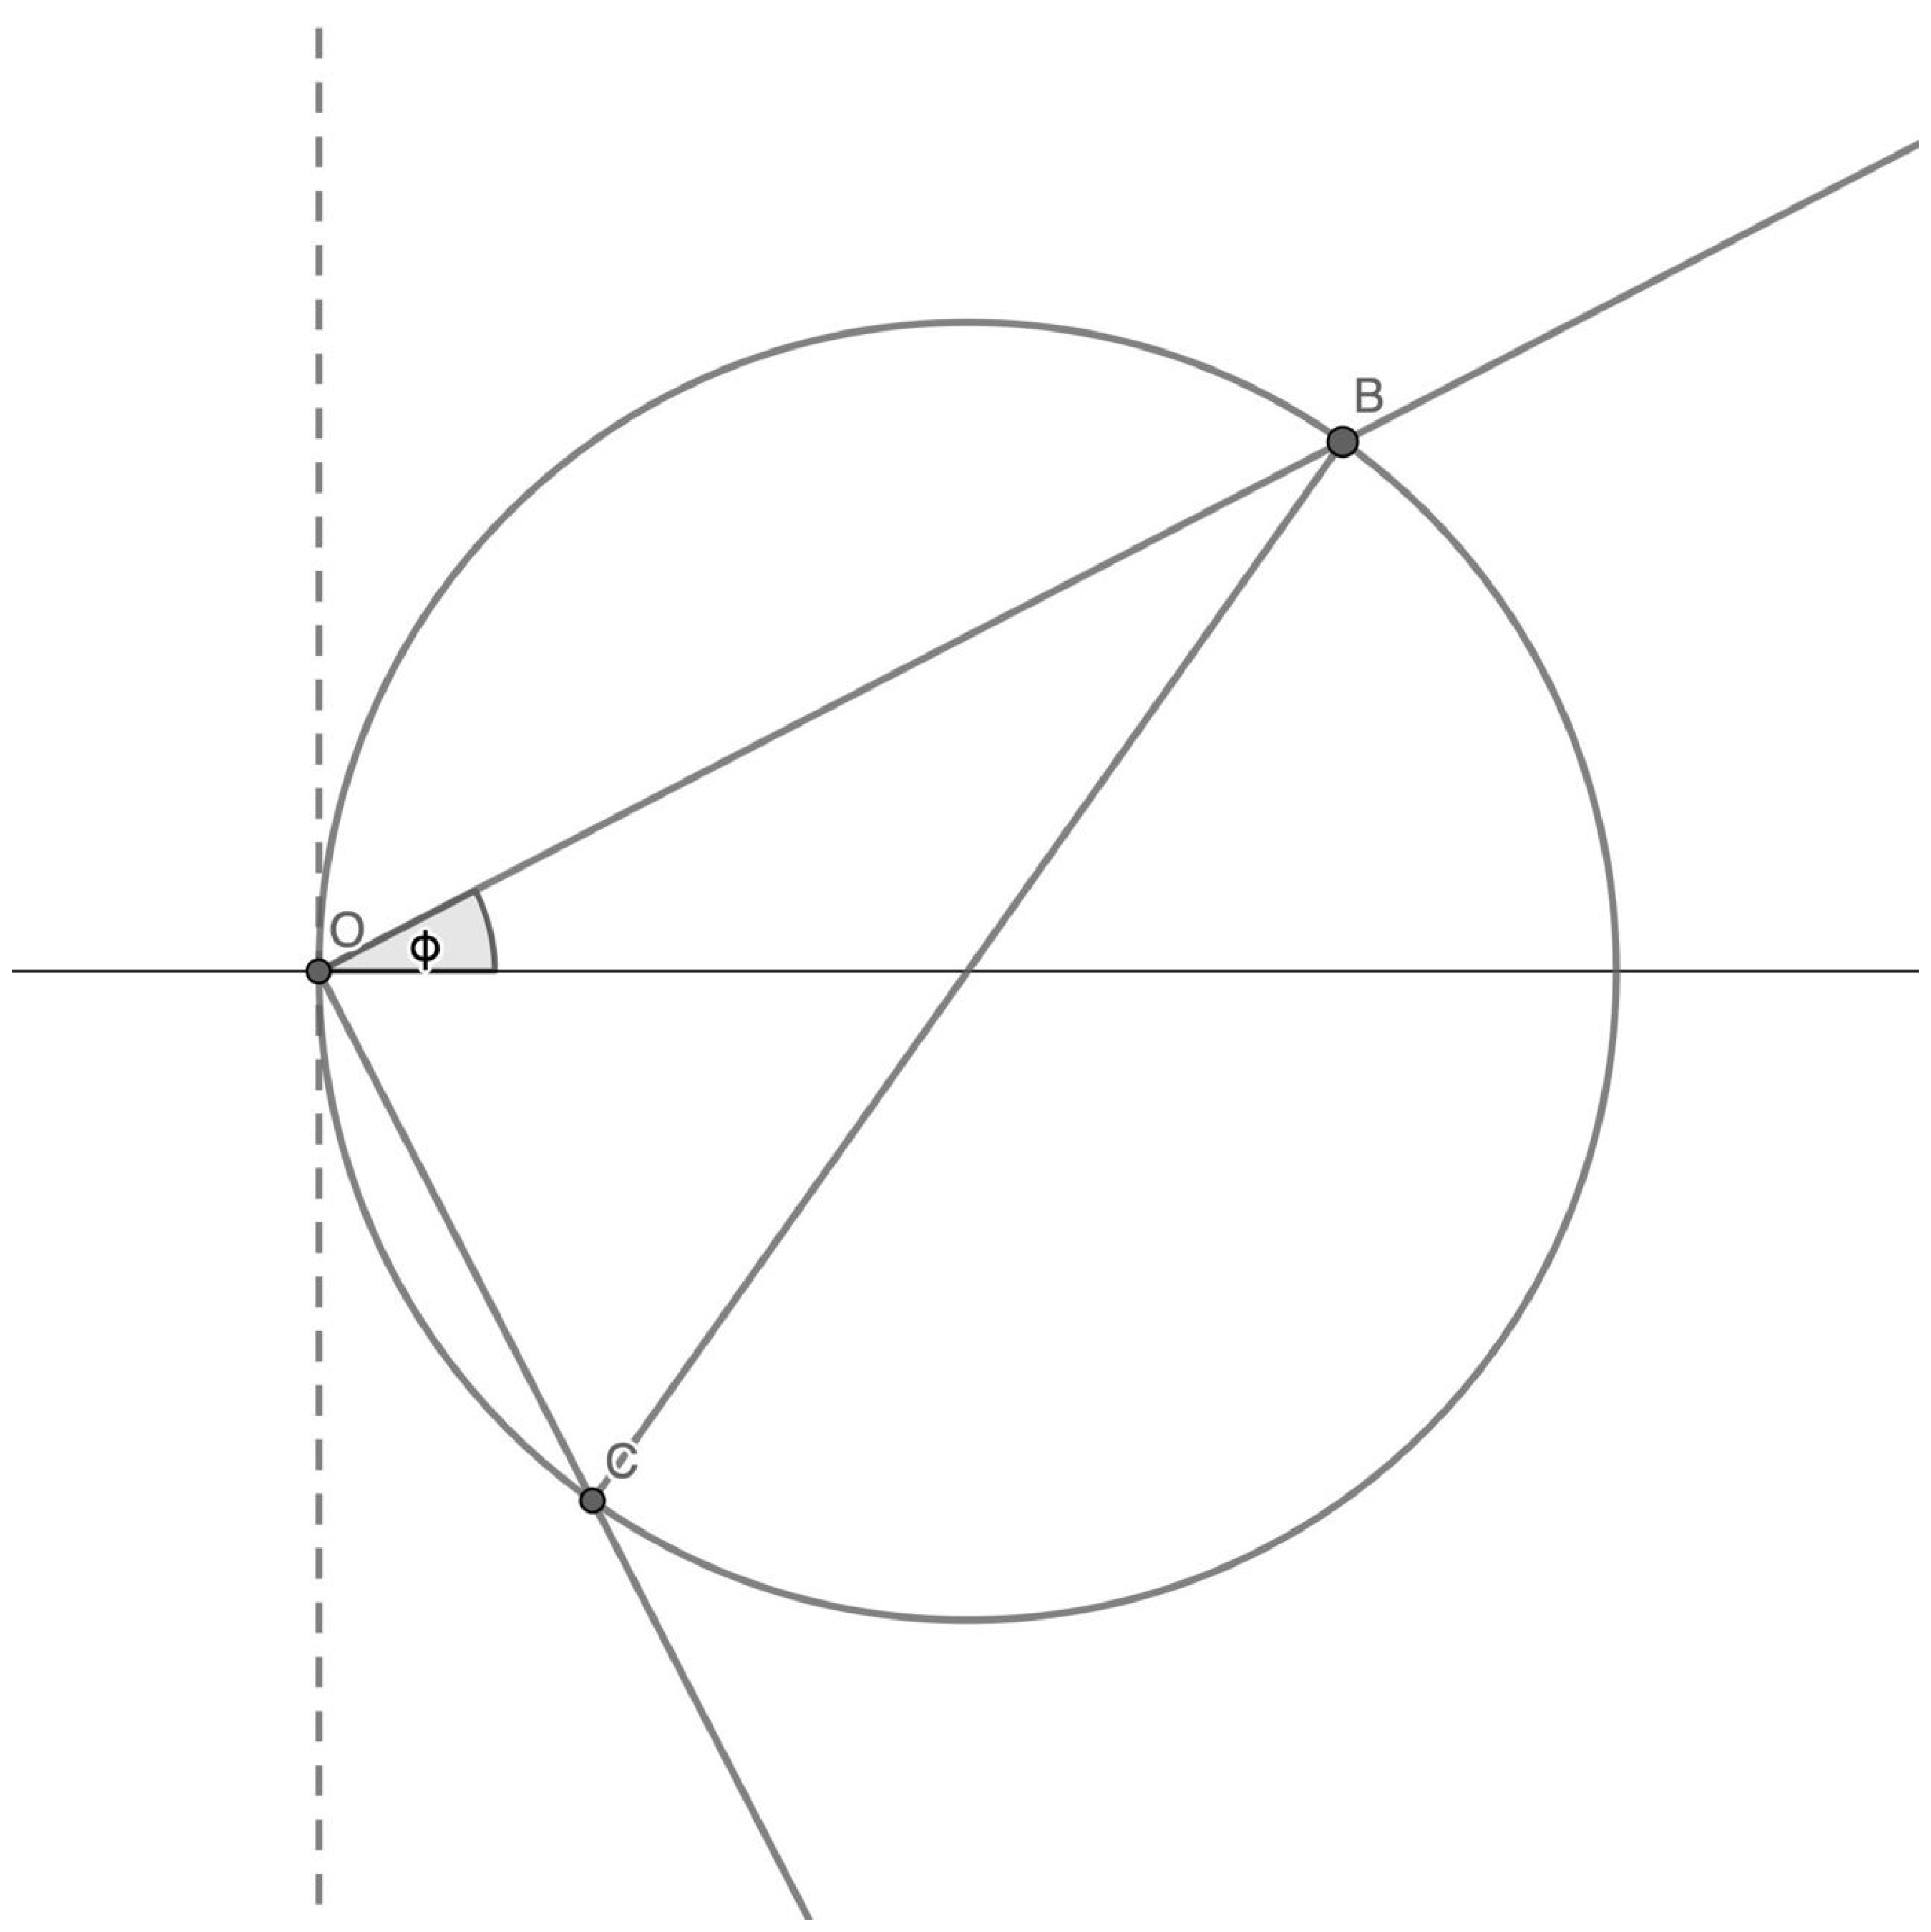
\includegraphics[width=0.5 \linewidth]{isoperimetric_3.eps}}
		\caption{Фокус}
	\end{figure}
	
	Тогда то, что на рисунке отмечено как \(OB\), это не что иное, как \(r(\varphi)\), а \(OC\) --- это \(r \left(\varphi - \dfrac{\pi}{2} \right)\). Но ведь \(OB\) и \(OC\) --- катеты прямоугольного треугольника, а значит \({OB}^2 + {OC}^2 = {BC}^2\). А так как \(BC \leqslant diam \ G \leqslant 1\), то и \(r^2(\varphi) + r^2 \left(\varphi - \dfrac{\pi}{2} \right) \leqslant 1\). А это, в свою очередь, значит, что \[
		\sigma(G) = \frac{1}{2} \int_{0}^{\frac{\pi}{2}} r^2 \left(\varphi - \frac{\pi}{2} \right) +  r^2(\varphi) d\varphi \leqslant \frac{1}{2} \int_{0}^{\frac{\pi}{2}} 1 d\varphi = \frac{\pi}{4}.
	\]
	
	ДОДЕЛАТЬ ПРО ПОЧТИ ДИФФЕРЕНЦИРУЕМОСТЬ (И МБ ПРО ВЫПУКЛЫЙ ПОДГРАФИК)
\end{proof}

\subsection{Обобщённая теорема о плотности}

\hypertarget{plotn}{}
\begin{theorem}
	Пусть \(\Phi \colon Segm \langle a, b \rangle \to \mathbb{R}\) --- аддитивная функция промежутка, функция \(f \colon \langle a, b \rangle \to \mathbb{R}\) непрерывна. Возьмём произвольный отрезок \(\Delta \in Segm \langle a, b \rangle\) и введём следующие обозначения: \(m_\Delta \leqslant \inf\limits_{x \in \Delta} f(x)\) и \(M_\Delta \geqslant \sup\limits_{x \in \Delta} f(x)\). Тогда если выполняются следующие условия:
	\begin{enumerate}
		\item \label{plotn_1} \(m_\Delta |\Delta| \leqslant \Phi(\Delta) \leqslant M_\Delta |\Delta|\),
		\item \label{plotn_2} \(\forall x \in \Delta \quad m_\Delta \leqslant f(x) \leqslant M_\Delta\),
		\item \label{plotn_3} \(\forall \Delta \mid |\Delta| \to 0 \quad M_\Delta - m_\Delta \to 0\)\footnote{То есть в контексте теоремы \(m_\Delta\) --- это слегка заниженный инфимум \(f\), а \(M_\Delta\) --- слегка завышенный супремум \(f\).},
	\end{enumerate}
	то \(f\) --- плотность функции \(\Phi\), то есть \[
		\forall [p, q] \in Segm \langle a, b \rangle \qquad \Phi([p, q]) = \int\limits_p^q f.
	\]
\end{theorem}

\begin{proof}
	Доказательство (как и теорема) очень-очень похоже на доказательство \hyperlink{afp}{теоремы о вычислении аддитивной функции промежутка по плотности}.
	
	Зафиксируем \([p, q] \in Segm \langle a, b \rangle\). Рассмотрим функцию \(F\): \[
	F(x) =
	\begin{cases}
		\Phi([p, x]), & p < x \leqslant q \\
		0,			  & x = p.
	\end{cases}
	\]
	Теперь проверим, что \(F\) --- первообразная \(f\) на \([p, q]\). Имеем: \[
	F'_+(x) = \lim_{h \to +0} \frac{\Phi([p, x + h]) - \Phi([p, x])}{h} = \lim_{h \to +0} \frac{\Phi([x, x + h])}{h}.
	\]
	Согласно пункту~\ref{plotn_1}, \(|\Delta| \cdot m_\Delta \leqslant \Phi(\Delta) \leqslant |\Delta| \cdot M_\Delta\), то есть \(m_\Delta \leqslant \dfrac{\Phi(\Delta)}{|\Delta|} \leqslant M_\Delta\), или
	\begin{equation} \label{plotn_e}
		m_{[x, x + h]} \leqslant \frac{\Phi([x, x + h])}{h} \leqslant M_{[x, x + h]}.
	\end{equation}
	Согласно пункту~\ref{plotn_2}, для всех \(x \) из \(\Delta\) справедливо \(m_\Delta \leqslant f(x) \leqslant M_\Delta\), то есть \(m_{[x, x + h]} \leqslant f(x) \leqslant M_{[x, x + h]}\), или \(-M_{[x, x + h]} \leqslant -f(x) \leqslant -m_{[x, x + h]}\). Сложим это неравенство с неравенством~\eqref{plotn_e}: \[
		m_{[x, x + h]} - M_{[x, x + h]} \leqslant \frac{\Phi([x, x + h])}{h} - f(x) \leqslant M_{[x, x + h]} - m_{[x, x + h]},
	\]
	Наконец, согласно пункту~\ref{plotn_3}, для любого \(\Delta \to [x, x]\) справедливо, что \(M_\Delta - m_\Delta \to 0\), то есть мы можем перейти к пределу: \[
		\lim_{h \to 0} m_{[x, x + h]} - M_{[x, x + h]} \leqslant \lim_{h \to 0} \frac{\Phi([x, x + h])}{h} - f(x) \leqslant \lim_{h \to 0} M_{[x, x + h]} - m_{[x, x + h]}.
	\]
	То есть \(F'_+(x) \to  f(x)\) при \(h \to 0\).
	
	Аналогично \(F'_-(x) = f(x)\). Применим \hyperlink{t9}{формулу Ньютона -- Лейбница} и получим требуемый результат: \[
	\Phi([p, q]) = F(q) - F(p) = \int_p^q f.
	\]
\end{proof}

\subsection{Объём фигур вращения}

\begin{theorem}
	ДОДЕЛАТЬ
\end{theorem}

\begin{proof}
	ДОДЕЛАТЬ
\end{proof}

\subsection{Вычисление длины гладкого пути}

\begin{theorem}
	Пусть \(\gamma \colon [a, b] \to \mathbb{R}^m\) --- гладкий путь, причём инъективный. Тогда \[
		l(\gamma) = \int\limits_a^b ||\gamma'(t)|| dt.
	\]
\end{theorem}

\begin{proof}
	Зафиксируем \(\Delta \in Segm [a, b]\) и рассмотрим функцию \(\Phi\), такую, что \(\Phi(\Delta) = l(\gamma |_\Delta)\). Заметим, что согласно аксиоме~\ref{way2} \(\Phi\) --- аддитивная функция промежутка. Тогда если мы докажем, что функция \(||\gamma'||\) --- плотность \(\Phi\), то, применив \hyperlink{plotn}{\bfseries обобщённую теорему о плотности}, мы докажем нашу теорему.
	
	Для этого мы должны проверить три условия из \hyperlink{plotn}{теоремы}. Сделаем это: для начала нужно предъявить слегка заниженный инфимум (минимум) \(m_\Delta\) и слегка завышенный супремум (максимум) \(M_\Delta\). Введём следующие обозначения:
	\begin{align*}
		m_{i\Delta} = \min\limits_{t \in \Delta} |\gamma'_i (t)|&, &&M_{i\Delta} = \max\limits_{t \in \Delta} |\gamma'_i (t)|, \\
		m_\Delta = \sqrt{\sum\limits_{i = 1}^m m_{i\Delta}^2}&, &&M_\Delta = \sqrt{\sum\limits_{i = 1}^m M_{i\Delta}^2},
	\end{align*}
	
	
	где \(i \in 1 : m\).\footnote{Минимум и максимум достигаются по теореме Вейерштрасса, так как функция \(|\gamma'_i(t)|\) непрерывна как композиция непрерывных функций, а рассматриваем мы её на отрезке.} Теперь начнём проверять необходимые условия:
	\begin{enumerate}
		\item Проверим справедливость верхней границы, справедливость нижней проверяется аналогичным образом. Введём \(\widetilde{\gamma} \colon \Delta \to \mathbb{R}^m\), такой, что \(\widetilde{\gamma}(t) = (M_{1\Delta} \cdot t, M_{2\Delta} \cdot t, \ldots, M_{m\Delta} \cdot t)\). Тогда \(C_{\gamma |_\Delta}\) и \(C_{\widetilde{\gamma}}\) --- носители наших путей. Рассмотрим отображение \(T \colon C_{\gamma |_\Delta} \to C_{\widetilde{\gamma}}\), которое переводит \(\gamma(t)\) в \(\widetilde{\gamma}(t)\). Проверим, что это растяжение: для любых  \(t_0, t_1 \in \Delta\) справедливо \[
			\rho(\gamma(t_0), \gamma(t_1)) =  \sqrt{\sum\limits_{i = 1}^m (\gamma_i (t_0) - \gamma_i (t_1))^2} = \ldots
		\]
		 Заметим, что по теореме Лагранжа \[
			\gamma_i (t_0) - \gamma_i (t_1) = \frac{\gamma_i (t_0) - \gamma_i (t_1)}{t_0 - t_1} (t_0 - t_1) = \gamma'_i(c_i) \cdot (t_0 - t_1), \ \text{где} \ c_i \in (t_0, t_1).
		\]
		Продолжим: \[
			\ldots =  \sqrt{\sum\limits_{i = 1}^m (\gamma'_i(c_i) \cdot (t_0 - t_1))^2} \leqslant \sqrt{\sum\limits_{i = 1}^m (M_{i\Delta} (t_0 - t_1) )^2} = \rho(\widetilde{\gamma}(t_0), \widetilde{\gamma}(t_1)).
		\]
		Мы доказали, что \(T\) --- растяжение, а сейчас нам полезно записать результат немного иным образом: для любых \(t_0, t_1 \in \Delta\) справедливо \[
			\rho(\gamma(t_0), \gamma(t_1)) \leqslant \rho(\widetilde{\gamma}(t_0), \widetilde{\gamma}(t_1)) = \sqrt{\sum\limits_{i = 1}^m (M_{i\Delta} (t_0 - t_1) )^2} = M_\Delta |t_0 - t_1|.
		\]
		Теперь мы можем выбрать любое дробление отрезка \(\Delta\) --- пусть \(\eta = \{t_0, t_1, \ldots, t_n\}\) --- и записать для него следующее неравенство: \[
			\sum_{i = 0}^n \rho(\gamma(t_i), \gamma(t_{i + 1})) \leqslant \sum_{i = 0}^n M_\Delta |t_i - t_{i + 1}| = M_\Delta \sum_{i = 0}^n |t_i - t_{i + 1}|.
		\]
		Если перейти к пределу при ранге дробления, стремящемся к нулю, неравенство выглядит так: \[
			\Phi(\Delta) \leqslant M_\Delta |\Delta|,
		\]
		а это как раз то, что мы хотели получить.
		\item Очевидно следует из определения введённых нами \(m_\Delta\) и \(M_\Delta\): при всех \(t \in \Delta\) \[
			m_\Delta \leqslant ||\gamma'(t)||\leqslant M_\Delta.
		\]
		\item Так как при \(|\Delta| \to 0 \ \max\limits_{t \in \Delta} |\gamma'_i (t)| - \min\limits_{t \in \Delta} |\gamma'_i (t)| \to 0\) для всех \(i \in 1 : m\), то и \(M_\Delta - m_\Delta \to 0\).
	\end{enumerate}
\end{proof}

\subsection{Теорема о функциях ограниченной вариации}

\begin{theorem}
	Пусть \(f\colon [a, b] \to \mathbb{R}\) --- \hyperlink{orgvar}{\bfseries функция ограниченной вариации}. Тогда существуют монотонные функции \(p, q\colon [a, b] \to \mathbb{R}\) такие, что для всех \(x \in [a, b]\) \(f(x) = p(x) - q(x)\).
\end{theorem}
\begin{proof}
	Возьмём такие \(p(x), q(x)\), что
	\begin{align*}
		2 \cdot p(x) &= \bigvee_a^x f + (f(x) - f(a)), \\
		2 \cdot q(x) &= \bigvee_a^x f - (f(x) - f(a)).
	\end{align*}
	Тогда имеем равенство \(f(x) - f(a) = p(x) - q(x)\). В принципе, это нам подходит, потому что \(f(a)\) --- константа, и мы можем прибавить её к \(p(x)\) или \(q(x)\), чтобы получить нужное равенство.
	
	Проверим теперь, что \(p\) и \(q\) возрастают, то есть что \(\bigvee_a^x f\) растёт быстрее, чем \(f(x)\). Пусть \(x < y\), запишем \[
		|f(y) - f(x)| \leqslant \bigvee_x^y f.
	\]
	Заметим, что функция \(\Phi\), переводящая \([u, v]\) в \(\bigvee_u^v f\), является аддитивной функцией промежутка (ДОДЕЛАТЬ). Тогда
	\begin{gather*}
		2 \cdot p(y) - 2 \cdot p(x) = \bigvee_x^y f + f(y) - f(x) \geqslant 0, \quad \text{то есть} \quad p(y) \geqslant p(x), \\
		2 \cdot q(y) - 2 \cdot q(x) = \bigvee_x^y f + f(x) - f(y) \geqslant 0, \quad \text{то есть} \quad q(y) \geqslant q(x).
	\end{gather*}
	Ну, вот и всё...
	
	И, \textit{кстати}, \(p(x) + q(x) = \bigvee_a^x f\).
\end{proof}

\subsection{\itshape Интеграл как предел интегральных сумм}

\begin{theorem}
	Пусть функция \(f \colon [a, b] \to \mathbb{R}\) непрерывна. Тогда
	\begin{gather*}
		\forall \varepsilon > 0 \quad \exists \delta > 0 \quad \forall \tau = \{x_i\}_{i = 0}^n \mid \text{ранг} \ \tau < \delta \quad \forall \text{оснащения} \ \{\xi_i\}_{i = 1}^n \ldots \\
		\ldots \left|\sum_{i = 1}^n f(\xi_i) (x_i - x_{i - 1}) - \int\limits_a^b f(x) dx \right| < \varepsilon.
	\end{gather*}
\end{theorem}

\begin{proof}
	Так как \(f\) непрерывна на отрезке, по теореме Кантора она равномерна непрерывна, то есть \[
		\forall \varepsilon > 0 \quad \exists \delta > 0 \quad \forall x_1, x_2 \mid |x_1 - x_2| < \delta \quad |f(x_1) - f(x_2)| < \frac{\varepsilon}{b - a}.
	\]
	Зафиксируем \(\varepsilon\) и подберём соответствующее \(\delta\). Возьмём дробление \(\tau\), ранг которого меньше \(\delta\).
	
	Теперь немного поработаем над нашими интегралом и суммой. Представим интеграл как сумму интегралов по отрезкам \([x_{i - 1}, x_i]\), а слагаемые интегральной суммы \(\sum\limits_{i = 1}^n f(\xi_i) (x_i - x_{i - 1})\) представим как интегралы константы \(f(\xi_i)\) по промежутку \([x_{i - 1}, x_i]\). Получим следующее: \[
		\sum_{i = 1}^n \int_{x_{i - 1}}^{x_i} f(\xi_i) dx - \sum_{i = 1}^n \int_{x_{i - 1}}^{x_i} f(x) dx = \sum_{i = 1}^n \int_{x_{i - 1}}^{x_i} f(\xi_i) - f(x) dx.
	\]
	То есть имеем \[
		\left|\sum_{i = 1}^n \int_{x_{i - 1}}^{x_i} f(\xi_i) - f(x) dx \right| \leqslant \sum_{i = 1}^n \int_{x_{i - 1}}^{x_i} \left|f(\xi_i) - f(x) \right| dx \leqslant \ldots
	\]
	Так как мы подобрали дробление с таким рангом, что для всех \(x \in [x_{i - 1}, x_i]\) и для любого оснащения \(\{\xi_i\}_{i = 1}^n \ |f(\xi_i) - f(x)| < \dfrac{\varepsilon}{b - a}\), можем продолжить цепочку неравенств: \[
		\ldots \leqslant \sum_{i = 1}^n \int_{x_{i - 1}}^{x_i} \frac{\varepsilon}{b - a} dx = \int\limits_a^b \frac{\varepsilon}{b - a} dx = \varepsilon.
	\]
\end{proof}

\subsection{Теорема об интегральных суммах центральных прямоугольников и трапеций}

\hypertarget{trap}{}
\begin{theorem}
	Пусть \(f \in C^2 [a, b]\), \(\tau = \{x_i\}_{i = 0}^n\) --- дробление отрезка \([a, b]\) с рангом \(\delta\). Выберем оснащение \(\{\xi_i\}_{i = 1}^n\), где \(\xi_i = \dfrac{x_i + x_{i - 1}}{2}\). Тогда справедливы следующие утверждения:
	\begin{gather}
		\label{intsum1}
		\left|\int\limits_a^b f(x) dx - \sum_{i = 1}^n f(\xi_i) (x_i - x_{i - 1}) \right| \leqslant \frac{\delta^2}{8} \int\limits_a^b |f''(x)| dx, \\
		\label{intsum2}
		\left|\int\limits_a^b f(x) dx - \sum_{i = 1}^n \frac{f(x_i) + f(x_{i - 1})}{2} (x_i - x_{i - 1})\right| \leqslant \frac{\delta^2}{8} \int\limits_a^b |f''(x)| dx.
	\end{gather}
\end{theorem}

\begin{proof}[Доказательство неравенства~\eqref{intsum2}]
	Рассмотрим интеграл на отрезке дробления и преобразуем его: \[
		\int_{x_{i - 1}}^{x_i} f(x) dx = \int_{x_{i - 1}}^{x_i} f(x) d(x - \xi_i) = \ldots
	\]
	Проинтегрируем его по частям: \[
		\ldots = f(x) (x - \xi_i) \bigg|_{x_{i - 1}}^{x_i} - \int_{x_{i - 1}}^{x_i} f'(x) (x - \xi_i) dx = \ldots
	\]
	Воспоминаем, что \(\xi_i = \dfrac{x_i + x_{i - 1}}{2}\): \[
		\ldots = \frac{f(x_i) + f(x_{i - 1})}{2} (x_i - x_{i - 1}) - \int_{x_{i - 1}}^{x_i} f'(x) (x - \xi_i) dx = \ldots
	\]
	Введём функцию \(\psi(x) = (x_i - x) (x - x_{i - 1})\) и рассмотрим её производную \(\psi'(x) = -(x - x_{i - 1}) + (x_i - x) = -2x + x_{i - 1} + x_i\). Заметим, что \(-\dfrac{1}{2} \psi'(x) = x - \xi_i\). Тогда продолжим: \[
		\ldots = \frac{f(x_i) + f(x_{i - 1})}{2} (x_i - x_{i - 1}) + \frac12 \int_{x_{i - 1}}^{x_i} f'(x) \cdot \psi'(x) dx = \ldots
	\]
	Опять проинтегрируем по частям:
	\begin{gather*}
		\ldots = \frac{f(x_i) + f(x_{i - 1})}{2} (x_i - x_{i - 1}) + \ldots \\
		\ldots + \frac{f'(x) \cdot \psi(x)}{2} \bigg|_{x_{i - 1}}^{x_i} - \frac{1}{2}\int_{x_{i - 1}}^{x_i} f''(x) \cdot \psi(x) dx = \ldots \\
		\ldots = \frac{f(x_i) + f(x_{i - 1})}{2} (x_i - x_{i - 1}) - \frac{1}{2}\int_{x_{i - 1}}^{x_i} f''(x) \cdot \psi(x) dx
	\end{gather*}
	
	Начнём разбираться с нашим неравенством:
	\begin{gather*}
		\left|\int\limits_a^b f - \sum_{i = 1}^n \textit{слагаемое}_i \right| = \left|\sum_{i = 1}^n \int_{x_{i - 1}}^{x_i} f - \sum_{i = 1}^n \textit{слагаемое}_i \right| = \ldots \\
		\ldots = \left|\sum_{i = 1}^n \int_{x_{i - 1}}^{x_i} f - \textit{слагаемое}_i \right| \leqslant \sum_{i = 1}^n \left|\int_{x_{i - 1}}^{x_i} f - \textit{слагаемое}_i \right|.
	\end{gather*}
	Воспользуемся нашими наработками:
	\begin{gather*}
		\sum_{i = 1}^n \left|\frac{f(x_i) + f(x_{i - 1})}{2} (x_i - x_{i - 1}) - \frac{1}{2}\int_{x_{i - 1}}^{x_i} f''(x) \cdot \psi(x) dx - \textit{слагаемое}_i \right| = \ldots \\
		\ldots = \frac{1}{2} \sum_{i = 1}^n \left|\int_{x_{i - 1}}^{x_i} f''(x) \cdot \psi(x) dx \right| \leqslant \frac{1}{2} \sum_{i = 1}^n \int_{x_{i - 1}}^{x_i} \left|f''(x) \cdot \psi(x) \right| dx = \ldots \\
		\ldots = \frac{1}{2} \int_a^b \left|f''(x) \cdot \psi(x) \right| dx.
	\end{gather*}
	
	Теперь оценим \(\psi(x)\). Рассмотрим \(\psi(\xi_i) = (x_i - \xi_i) (\xi_i - x_{i - 1})\): \[
		\psi(\xi_i) = \left(x_i - \frac{x_i + x_{i - 1}}{2} \right) \left(\frac{x_i + x_{i - 1}}{2} - x_{i - 1}\right) = \left(\frac{x_i - x_{i - 1}}{2} \right)^2.
	\]
	Так как ранг дробления \(\tau\) равен \(\delta\), справедливо: \[
		\psi(\xi_i) \leqslant \frac{\delta^2}{4}.
	\]
	Тогда \[
		\frac{1}{2} \int_a^b \left|f''(x) \cdot \psi(x) \right| dx \leqslant \frac{\delta^2}{8} \int_a^b \left|f''(x) \right| dx.
	\]
\end{proof}

